\documentclass[stu]{apaV7}
\usepackage[spanish,es-tabla]{babel}
\usepackage{csquotes}
\usepackage{lipsum}
\usepackage[style=apa,sortcites=true,sorting=nyt,backend=biber]{biblatex}
%\DeclareLanguageMapping{american}{american-apa}
\addbibresource{bibliography.bib}

%\hypersetup{nolinks=true}

\title{Titulo del articulo apa 7 estudiante}
\author{Yoel Antony Medina Jacho}
\affiliation{Universidad Nacional de San Agustin}
\course{Curso de Universidad}
\professor{el Profesor pe}
\duedate{\today}
\abstract{\lipsum[3]}
\keywords{primero, segundo, tercero}
\abstractEng{Resumen pero en ingles\lipsum[3]}
\keywordsEng{First, segundo, tercero}



\begin{document}
	
	\maketitle
	
	
	Introduccion para el articulo \lipsum[2]
	\section{M\'etodo}
	\subsection{Participantess}
	\lipsum[4]
	
	\Textcite{vonDavier2011} said this,
	too \parencite{vonDavier2011,Lassen2006}.  Further evidence comes from
	other sources \parencite{Shotton1989,Lassen2006}.  \lipsum[3]
	
	\subsection{Materiales}
	\lipsum[5]
	
	\subsection{Design}
	\lipsum[6]
	
	\subsection{Procedure}
	\lipsum[7]
	
	\subsubsection{Instrumento \#1}
	\lipsum[8]
	
	\paragraph{Reliability}
	\lipsum[9]
	
	\subparagraph{Inter-rater reliability}
	\lipsum[10]
	
	\subparagraph{Test-retest reliability}
	\lipsum[11]
	
	\paragraph{Validity}
	\lipsum[12]
	
	\subparagraph{Face validity}
	\lipsum[13]
	
	\subparagraph{Construct validity}
	\lipsum[14]
	
	\section{Results}
	Tabla~\ref{tab:BasicTable} summarizes the data. \lipsum[15]
	
	\begin{table}
		\caption{Sample B\'asico Tabla}
		\label{tab:BasicTable}
		\begin{tabular}{@{}llr@{}}         \toprule
			\multicolumn{2}{c}{Item}        \\ \cmidrule(r){1-2}
			Animal    & Description & Price \\ \midrule
			Gnat      & per gram    & 13.65 \\
			& each        &  0.01 \\
			Gnu       & stuffed     & 92.50 \\
			Emu       & stuffed     & 33.33 \\
			Armadillo & frozen      &  8.99 \\ \bottomrule
		\end{tabular}
	\end{table}
	
	\begin{figure}
		\caption{This is my first figure caption.}
		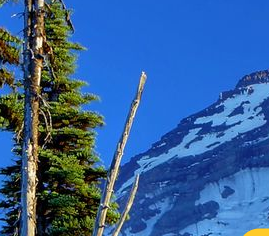
\includegraphics[bb=0in 0in 2.5in 2.5in, height=2.5in, width=2.5in]{Figure1.png}
		\label{fig:Figure1}
	\end{figure}
	
	Figure~\ref{fig:Figure1} shows this trend. \lipsum[16]
	
	\section{Discussion}
	\lipsum[17]
	
	\printbibliography


%\appendix

%\section{Instrument}
%\label{app:instrument}

%As shown in Figure~\ref{fig:Figure2}, these results are impressive. \lipsum[20]

%\begin{figure}
%	\caption{This is my second figure caption.}
%	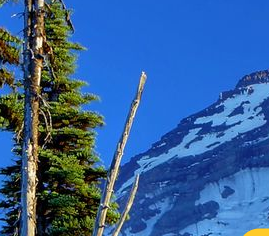
\includegraphics[bb=0in 0in 2.5in 2.5in, height=2.5in, width=2.5in]{Figure1.png}
%	\label{fig:Figure2}
%\end{figure}

%\lipsum[21]
%\section{Pilot Data}
%\label{app:surveydata}

%The detailed results are shown in Table~\ref{tab:DeckedTable}. \lipsum[22]

%\lipsum[23]

\end{document}
